\section{Deep-inelastic scattering with LHC neutrinos}
\label{sec:dis_pseudodata}

Here we describe the procedure adopted in order 
to generate projections for the kinematic coverage
and uncertainties associated to  measurements
of neutrino-nucleus scattering at the LHC far-forward experiments.
%
First, we summarise the theoretical description of differential
neutrino scattering in terms of DIS structure functions and highlight
their PDF sensitivity.
%
Second, we present an  overview of the operative and proposed
LHC far-forward neutrino detectors that
will be considered in the present study and indicate their
acceptance and performance parameters.
%
By convoluting the expected electron and muon neutrino fluxes
with the acceptance and scattering rates of each
of these detectors,
we evaluate the event yields in bins of $x$, $Q^2$,
and $E_\nu$ and the associated statistical and systematic uncertainties.
%
Finally, we discuss the procedure adopted to generate pseudo-data
for LHC neutrino deep-inelastic scattering structure functions
and to quantify their impact
 into proton and nuclear PDF determinations.

 \subsection{Neutrino DIS revisited}
 \label{sec:nudis_revisited}

The double-differential cross-section for neutrino-nucleus charged-current scattering,
see~\cite{Candido:2023utz} and references therein,
is expressed in terms of three
independent structure functions $F_2^{\nu A}$, $xF_3^{\nu A}$
and $F_L^{\nu A}$:
\be
\label{eq:neutrino_DIS_xsec_FL}
\frac{d^2\sigma^{\nu A}(x,Q^2,y)}{dxdy} =  \frac{G_F^2s/4\pi}{\lp 1+Q^2/m_W^2\rp^2}\lc Y_+F^{\nu A}_2(x,Q^2) - y^2F^{\nu A}_L(x,Q^2) +Y_- xF^{\nu A}_3(x,Q^2)\rc  \, ,
\ee
where $Y_\pm = 1 \pm (1-y)^2$ and with a counterpart expression for anti-neutrino scattering,
\be
\label{eq:antineutrino_DIS_xsec_FL}
\frac{d^2\sigma^{\bar{\nu} A}(x,Q^2,y)}{dxdy} =  \frac{G_F^2s/4\pi}{\lp 1+Q^2/m_W^2\rp^2}\lc Y_+F^{\bar{\nu} A}_2(x,Q^2) - y^2F^{\bar{\nu} A}_L(x,Q^2) -Y_- xF^{\bar{\nu} A}_3(x,Q^2)\rc  \, ,
\ee
where $s=2m_N E_\nu$ being the neutrino-nucleon center of mass energy squared, $m_N$ is the nucleon mass,
$E_\nu$ is the incoming neutrino energy,
and the inelasticity is $y=Q^2/(2x m_n E_{\nu})$.
%
In the case of tau-neutrino scattering, tau lepton mass effects
cannot be neglected and Eqns.~(\ref{eq:neutrino_DIS_xsec_FL}) and~(\ref{eq:antineutrino_DIS_xsec_FL}) receive additional contributions
from the $F_4$ and $F_5$ structure functions.
%
We neglect these effects since we focus on electron and muon neutrino scattering here.

Structure functions depend only on $x$ and $Q^2$, while the differential
cross-section depends also on the neutrino energy $E_\nu$, or alternatively
on the inelasticity $y$.
%
Further, structure functions $F^{\nu A}_i(x,Q^2)$ and $F^{\bar{\nu} A}_i(x,Q^2)$ depend on the nuclear target $A$ entering
for the neutrino scattering through the nuclear modifications of the free-nucleon PDFs.
%
Eqns.~(\ref{eq:neutrino_DIS_xsec_FL}) and~(\ref{eq:antineutrino_DIS_xsec_FL}) are valid provided
the hadronic 
invariant mass $W$  is above the resonance production threshold,
\be
W^2 = \lp m_N^2 + Q^2 \frac{(1-x)}{x} \rp \gsim \lp 2\,{\rm GeV} \rp^2\, ,
\ee
and in addition here we  restrict ourselves to the DIS region with perturbative momentum
transfers $Q^2 \gsim 2$ GeV$^2$, such that
 structure functions can be decomposed as
\be
\label{eq:sfs_pqcd}
 F^{\nu A}_i(x,Q^2) = \sum_{j=q,\bar{q},g}\int_x^1 \frac{dz}{z}\, C_{i,j}^{\nu N}(z,\alpha_s(Q^2))f^{(A)}_j\lp \frac{x}{z},Q^2\rp \, , \quad i = 2,3,L \, .
 \ee
%
in terms of a convolution of partonic scattering cross-sections  $C_{i,j}^{\nu N}(x,\alpha_s)$ and
of process-independent PDFs $f^{(A)}_j\lp x,Q^2\rp$.
%
A similar expression holds for charm production~\cite{Faura:2020oom}, which requires
accounting also for charm mass effects~\cite{Gao:2017kkx}.
 %
We discuss below the theoretical
settings adopted here~\cite{Candido:2022tld,yadism,Candido:2023utz,Carrazza:2020gss} to
evaluate predictions for
neutrino differential cross-sections and DIS structure functions,
Eqns.~(\ref{eq:neutrino_DIS_xsec_FL}),~(\ref{eq:antineutrino_DIS_xsec_FL}), and~(\ref{eq:sfs_pqcd}),
in the kinematics covered by LHC neutrinos.

Different neutrino structure functions provide complementary sensitivity
 to the partonic flavour decompositions of nucleons.
 %
 To illustrate this sensitivity, consider a leading order  calculation
 for a proton target with $n_f=4$ active quark flavours,
a diagonal CKM matrix and no heavy quark mass effects.
 %
 The resulting $F_2^{\nu p}$ and $xF_3^{\nu p}$ structure functions read
 \bea
 F_2^{\nu p}(x,Q^2) &=& 2x\lp f_{\bar{u}} + f_{d} + f_{s} + f_{\bar{c}} \rp(x,Q^2) \, , \nonumber  \\
 F_2^{\bar{\nu} p}(x,Q^2) &=& 2x\lp f_u + f_{\bar{d}} + f_{\bar{s}} + f_c \rp(x,Q^2) \, , \label{eq:neutrinoSFs_proton} \\
 xF_3^{\nu p}(x,Q^2) &=& 2x\lp -f_{\bar{u}} + f_d +f_s - f_{\bar{c}}\rp(x,Q^2)  \, , \nonumber\\
 xF_3^{\bar{\nu} p}(x,Q^2) &=& 2x\lp f_u - f_{\bar{d}} -f_{\bar{s}} + f_{c}\rp(x,Q^2) \, . \nonumber
 \eea
 The corresponding expressions for a neutron target are obtained from isospin symmetry
 \bea
 F_2^{\nu n}(x,Q^2) &=& 2x\lp f_{\bar{d}} + f_{u} + f_{s} + f_{\bar{c}} \rp(x,Q^2) \, , \nonumber  \\
 F_2^{\bar{\nu} n}(x,Q^2) &=& 2x\lp f_d + f_{\bar{u}} + f_{\bar{s}} + f_c \rp(x,Q^2) \, , \label{eq:antineutrinoSFs_neutron} \\
 xF_3^{\nu n}(x,Q^2) &=& 2x\lp -f_{\bar{d}} + f_u +f_s - f_{\bar{c}}\rp(x,Q^2)  \, , \nonumber\\
 xF_3^{\bar{\nu} n}(x,Q^2) &=& 2x\lp f_d - f_{\bar{u}} -f_{\bar{s}} + f_{c}\rp(x,Q^2) \, , \nonumber
 \eea
 while for an isoscalar, free-nucleon target denoted by $N$ one has
 \bea
 F_2^{\nu N}(x,Q^2) &=& 2x\lp f_{u^+} + f_{d^+} + 2f_s + 2f_{\bar{c}} \rp(x,Q^2) \, , \nonumber  \\
 F_2^{\bar{\nu} N}(x,Q^2) &=& 2x\lp f_{u^+} + f_{d^+} + 2f_{\bar{s}} + 2f_c \rp(x,Q^2) \, , \label{eq:neutrinoSFs_isoscalar} \\
 xF_3^{\nu N}(x,Q^2) &=& 2x\lp f_{u^-} + f_{d^-} +2f_s - 2f_{\bar{c}}\rp(x,Q^2)  \, , \nonumber\\
 xF_3^{\bar{\nu} N}(x,Q^2) &=& 2x\lp   f_{u^-} + f_{d^-}-2f_{\bar{s}} +2 f_{c}\rp(x,Q^2) \, , \nonumber
 \eea
 in terms of the valence and sea PDF combinations defined by
 \be
 f_{q^+} (x,Q^2)\equiv \lp f_{q}+f_{\bar{q}}\rp(x,Q^2) \, , \qquad
 f_{q^-} (x,Q^2)\equiv \lp f_{q}- f_{\bar{q}}\rp(x,Q^2) \, .
 \ee
 We note that, even for isoscalar targets, separate measurements
 for neutrinos and antineutrinos will not be equivalent, since in general
 the strange and charm sea asymmetries $f_{s^-}$ and
 $f_{c^-}$ are not expected to vanish.

 In the projections presented in this work, when interpreting the LHC neutrino structure
 functions in terms of proton PDFs, we will assume a isoscalar free-nucleon target and neglect
 nuclear PDF modifications, along the lines of Eq.~(\ref{eq:neutrinoSFs_isoscalar}).
 %
 On the other hand, when evaluating structure functions
 for a tungsten (W) target, we keep into account both
 nuclear corrections and that
 the target is not isoscalar when evaluating the physical observables.
 %
 Accounting for nuclear modifications in a global proton
 PDF fit is possible by means of the procedure developed
 in~\cite{Ball:2020xqw,Ball:2018twp} based on
 the theory covariance matrix approach~\cite{NNPDF:2019vjt,NNPDF:2019ubu}.

 It is illustrative to compare the PDF dependence of neutrino structure functions
 at LO with that of their counterparts for neutral-current
 scattering with a charged lepton projectile.
 %
 Within the same assumptions, for energies below
 the $Z$-boson mass, $Q^2 \ll m_Z^2$, the corresponding
 partonic decomposition is
 the 
 \bea
 F_2^{\ell p}(x,Q^2) &=& x\lp \frac{4}{9}\lc f_{u^+} + f_{c^+}\rc
 + \frac{1}{9}\lc f_{d^+} + f_{s^+}\rc\rp(x,Q^2) \, , \nonumber  \\
 F_2^{\ell n}(x,Q^2) &=& x\lp \frac{4}{9}\lc f_{d^+} + f_{c^+}\rc
 + \frac{1}{9}\lc f_{u^+} + f_{s^+}\rc\rp(x,Q^2) \, ,\label{eq:NC_chargedlepton}   \\
 F_2^{\ell N}(x,Q^2) &=& x\lp \frac{5}{18}\lc f_{u^+} + f_{d^+}\rc
 + \frac{1}{9} f_{s^+} + \frac{4}{9} f_{c^+} \rp(x,Q^2) \, , \nonumber  
 \eea
 with $xF_3$ being negligible in this region below the $Z$-pole.
 %
 Eq.~(\ref{eq:NC_chargedlepton}) showcases the complementarity between
 neutrino and charged-lepton DIS in terms of sensitivity
 to the different flavour PDF decomposition.
 %
 This implies that the best sensitivity on the quark
  flavour separation in the nucleon
 would be provided by combining neutrino DIS at
 LHC far-forward experiments with measurements on charged-lepton
 DIS at the EIC.

 \subsection{LHC far-forward neutrino detectors}
 \label{sec:neutrinoDetectors}

 The calculation of differential neutrino scattering event rates
 at the LHC far-forward detectors involves two main ingredients: the energy
 and flavour dependence of the incoming neutrino flux crossing
 the detector fiducial volume, on the one hand,
 and the scattering rates within the same fiducial volume, on the other hand.
 %
 Here we summarise the main features of each of the existing and future
 far-forward detectors considered, in particular concerning
 their acceptance and (expected) performance.
 %
 We focus on  muon neutrino scattering, which benefits from the highest rates and is less
 affected by theoretical uncertainties in the production mechanism.
 
 The kinematics of a charged-current neutrino DIS event $(x,Q^2, E_\nu)$,
 or alternatively $(x,Q^2, y)$, are uniquely specified by the measurement of three independent
 final-state variables,
 such as $\lp E_\ell,\theta_\ell, W^2\rp$ or $\lp E_\ell,\theta_\ell, E_h \rp$,
 with $E_\ell$ and $\theta_\ell$ being the energy and polar angle of the outgoing
 charged lepton and $E_h$ the total energy of the hadronic final state.
 %
 Most neutrino detectors can only access $E_h$, given that $W^2$ requires
 fully reconstructing this final state.
 %
 A measurement of the three kinematic variables $\lp E_\ell,\theta_\ell, E_h \rp$ then fixes the DIS kinematics as:
 \bea
 E_\nu &=& E_h + E_\ell \, , \nonumber \\
 Q^2 &=& 4 ( E_h + E_\ell) E_\ell \sin^2 \lp \theta_\ell/2\rp \, ,  \label{eq:dis_kinematic_mapping}\\
 x&=& \frac{4 ( E_h + E_\ell) E_\ell \sin^2 \lp \theta_\ell/2\rp}{2m_N E_h} \, .\nonumber
 \eea
 These relations also indicate how systematic uncertainties affecting the measurement
 of $\lp E_\ell,\theta_\ell, E_h \rp$ translate into uncertainties in the
 reconstructed values of  $(x,Q^2, E_\nu)$ modifying the expected
 binned event rates.

 Table~\ref{tab:FPF_experiments} summarises,
 for each of the far-forward LHC neutrino experiments considered in this
 work,
 their pseudo-rapidity coverage, target material, whether
  they can identify the sign of the outgoing charged lepton,
  the acceptance for the charged lepton and hadronic final state,
  and the expected reconstruction performance.
  %
  We consider separately acceptance and performance for electron and muon
  neutrinos.
  %
  For these projections we assume that FASER$\nu$ and SND@LHC acquire data
  for Run III ($\mathcal{L}=150$ fb$^{-1}$), while FASER$\nu$2,
  AdvSND, and FLArE take data
  for the complete HL-LHC period  ($\mathcal{L}=3$ ab$^{-1}$).
  %
   In the case of FLArE, we consider projections for both
  for 10 ton and 100 fiducial volume detectors.
  %
  In the following we provide more details about the information collected in
  Table~\ref{tab:FPF_experiments}.

%---------------------------------------------------
    %-----------------------------------------------------------------
\begin{table}[t]
  \centering
  \small
  \renewcommand{\arraystretch}{1.50}
\begin{tabularx}{\textwidth}{Xccccc}
\toprule
Detector &  Rapidity &  Target & Charged Lepton ID & Acceptance  & Performance \\
\midrule
\midrule
\multirow{3}{*}{FASER$\nu$}  &  \multirow{3}{*}{ $\eta_\nu \ge 8.5$}  &   \multirow{2}{*}{Tungsten}  & \multirow{3}{*}{muons}      &   $E_\ell \gsim 100$ GeV   &      $\delta E_\ell \sim 30\% $    \\
&   &   \multirow{2}{*}{(1.1 ton)}  &       &  $\tan \theta_\ell \lsim 0.025$   &
$\delta \theta_\ell \sim 0.06$ mrad        \\
&   &     &       &  reconstructed $E_h$ \& charm ID   &      $\delta E_h \sim 30\%$     \\
\midrule
\multirow{2}{*}{SND@LHC}  & \multirow{2}{*}{ $7.2 \le \eta_\nu \le 8.4$}   &  Tungsten   &   \multirow{2}{*}{n/a}    &  $E_\mu \gsim 20 $ GeV     &    \multirow{2}{*}{n/a}    \\
  &    &  (0.83 ton)   &  &  $\theta_\mu \lsim 0.15, \theta_e \lsim 0.5$         &       \\
\midrule
\midrule
\multirow{3}{*}{FASER$\nu$2}  & \multirow{3}{*}{ $\eta_\nu \ge 8.5$}  & \multirow{2}{*}{Tungsten}    &   \multirow{3}{*}{muons}     &   $E_\ell \gsim 100$ GeV  &    $\delta E_\ell \sim 30\% $     \\
  &   &  \multirow{2}{*}{(20 ton)}   &       &  $\tan \theta_\ell \lsim 0.05$   &   $\delta \theta_\ell \sim 0.06$ mrad      \\
  &   &     &       &  reconstructed $E_h$ \& charm ID   &  $\delta E_h \sim 30\%$        \\
\midrule
\multirow{3}{*}{AdvSND-far}  &   \multirow{3}{*}{ $7.2 \le \eta_\nu \le 8.4$}  &
\multirow{2}{*}{Tungsten}   &   \multirow{3}{*}{muons}    &  $E_\mu \gsim 20 $ GeV  & \multirow{3}{*}{n/a}          \\
  &   &   \multirow{2}{*}{(5 ton)}  &        & $\theta_\mu \lsim 0.15, \theta_e \lsim 0.5$     &           \\
  &   &     &       &  reconstructed $E_h$   &           \\
\midrule
\multirow{3}{*}{FLArE ({\bf *})}  & \multirow{3}{*}{$\eta_\nu \ge 7.5$} & \multirow{2}{*}{LAr}  & \multirow{3}{*}{muons}  &  $E_\mu \gsim 2$ GeV, $E_e \lsim 2$ TeV    &    $\delta E_e \sim 5\% $ \\
&   &  \multirow{2}{*}{(10 ton)}   &   & $\theta_\mu \lsim 0.025$, $\theta_e \lsim 0.5$ &    $\delta \theta_e \sim 15 $ mrad   \\
 &   &     &  & reconstructed $E_h$  &    $\delta E_h \sim 30\% $   \\
  \bottomrule
\end{tabularx}
\vspace{0.2cm}
\caption{\small For each of the far-forward LHC neutrino experiments considered
   we indicate their neutrino pseudo-rapidity coverage, target material, whether
  they can identify the sign of the outgoing charged lepton,
  the acceptance for the charged lepton and hadronic final state,
  and the expected reconstruction performance.
  %
  We consider separately acceptance and performance for electron and muon
  neutrinos.
  %
  For FLArE, we assume that muons would be measured in the FASER2 spectrometer
  situated downstream in the FPF cavern.
  %
  See the description of each experiment in the text for more details.
  %
  For our projections we assume that FASER$\nu$ and SND@LHC acquire data
  for the Run III period ($\mathcal{L}=150$ fb$^{-1}$), while FASER$\nu$2, AdvSND, and FLArE take data
  for the complete HL-LHC period ($\mathcal{L}=3$ ab$^{-1}$).
  %
  In the case of FLArE, we consider results both
  for 10 ton and 100 fiducial volume detectors.
  \label{tab:FPF_experiments}
}
\end{table}
%-----------------------------------------------------------------

%---------------------------------------------------

\paragraph{FASER$\nu$.}
%
The ForwArd Search ExpeRiment (FASER) detector
and its companion FASER$\nu$~\cite{FASER:2019aik,FASER:2019dxq,FASER:2023zcr,FASER:2022hcn}
are located at the TI12 tunnel of the CERN accelerator complex.
%
Both detectors are aligned
with the collision axis line-of-sight (LOS)
and have been acquiring data since the beginning of Run III in 2022.
%
Neutrino scattering takes place in the FASER$\nu$ 
detector, composed by interleaved emulsion and tungsten plates and
adding up to a mass of 1.1 tons with a fiducial volume of $20~\rm{cm} \times 25~\rm{cm} \times 80~{\rm cm}$.
%
The FASER apparatus is immersed in a magnetic field  providing charged lepton
identification thanks to two 1 m-long dipole magnets with $B=0.57$ T
and another 1.5 m-long magnet in front of the spectrometer. 
%
Neutrino detection and identification can be carried out either using the emulsion
films, which have the key benefit of excellent position and angular resolution,
or instead using the electronic detector components of FASER, which enable the tagging
of the outgoing downstream energetic muons.
%
FASER$\nu$ is sensitive to neutrinos with pseudorapidity $\eta_\nu \ge 8.5$
and can also identify charm-tagged events.


\paragraph{SND@LHC.}
%
In the same manner as FASER, the SND@LHC experiment~\cite{SNDLHC:2022ihg}
is located in a service tunnel (TI18)
around 500 meters from the ATLAS interaction point and has been taking data
since the  beginning of Run III.
%
SND@LHC is installed off the LOS axis in order to cover the neutrino
pseudo-rapidity range of $7.2 \le \eta_\nu \le 8.4$.
%
With a total fiducial volume of 830 kg and length of 35 cm, it is composed by tungsten plates,
where neutrino scattering takes place, interleaved with nuclear emulsions and electronic tracker
components.
%
Downstream, the scattering volume is followed by a hadronic calorimeter and a muon tracking system.
%
The electromagnetic
 and hadronic energy deposits can be measured at the electronic detectors, with the emulsion
 components providing vertex reconstruction.
 %
 The lack of magnetic field prevents the charge-sign identification of the outgoing charged leptons.

\paragraph{FASER$\nu$2.}
%
A proposed 20-ton neutrino experiment located on the LOS
of the LHC neutrino beam to be installed in the FPF cavern.
%
It is based on the same technology as FASER$\nu$, and hence
relies on a emulsion-based detector optimised to identify heavy flavor particles, including
tau leptons and charm and beauty particles, arising from neutrino interactions.
%
It would be sensitive to neutrinos with pseudorapidity $\eta_\nu \ge 8.5$.
%
The FASER$\nu$2 detector is composed of 3300 emulsion layers interleaved with 2-mm-thick tungsten plates,
for a total volume of  tungsten of $40~\rm{cm} \times 40~\rm{cm} \times 6.6~{\rm m}$.
%
The combination of FASER$\nu$2  with the nearby FASER2 detector, equipped with a spectrometer, makes measurements of the outgoing muon charge possible.
%
Given that FASER$\nu$2 is based on the same detector technology
as its predecessor, the same performance in terms of reconstruction
of final-state kinematics is assumed.

 \paragraph{AdvSND.}
 %
 This proposed experiment consists actually on  two detectors, a far-detector to be installed
 at the FPF with a coverage in neutrino pseudorapidity of $7.2 \le \eta_\nu \le 8.4$
 (hence off-LOS, same as SND@LHC) and a near detector installed somewhere else in LHC
 complex and covering the range $4 \le \eta_\nu \le 5$.
 %
 In the following we focus on the AdvSND-far detector.
 %
 It would be
 composed (from upstream to downstream) by a target region
 for  vertex reconstruction and electromagnetic energy measurement, followed  by a hadronic calorimeter, a  muon 
 identification system, and finally  a magnet enabling muon charge and momentum measurements.
 %
 The target region of the detector, where the neutrino interactions take place, is made of thin sensitive layers 
 interleaved with tungsten plates, for a total mass of 5 tons and fiducial length of 50 cm.
 %
 This detector configuration will be able to track muons with energy $E_\nu \gsim 20$ GeV
 within an acceptance of 100 mrad and provide information on the charge
 of the  outgoing muon thanks to its magnet.
 %
 The total energy of the hadronic final state will be measured
 in the hadronic calorimeter.
 %
 No information on the expected performance of the AdvSND-far detector
 is available and hence no estimate of the systematic errors
 is carried out.

 \paragraph{FLArE.}
 %
 Building upon recent progress in liquid noble gas neutrino detectors over the last decade (ICARUS, MicroBooNE, SBND, ProtoDUNE, DUNE), this experiment
 would rely on a modularized liquid argon (LAr) time projection detector.
 %
 The use of LAr as a target is beneficial for final-state particle identification, track angle, and kinetic energy measurements with sub-millimeter spatial resolution in all dimensions.
 %
% FLArE is suitable to identify high-energy neutrinos ($E_\nu \gsim 100$ GeV)  from all three generations while containing the events as required for kinematic reconstruction.
 %
 The detector will be equipped with a magnetized hadron/muon calorimeter downstream of the liquid argon volume
 for muon charge and momentum measurements.
 %
 While muon neutrinos with energy $E_\nu \gsim 2$ GeV would not be fully
 contained in the  FLArE detector,
for the projections presented in this work
we assume that outgoing high-energy
muons would be measured in the FASER2 spectrometer
  situated downstream in the FPF cavern.
 
 With an expected fiducial (active) mass of 10 tons (30 tons) and length 7 m, FLArE will
 detect final-state electrons with energies $E_{e}\lsim 2~\rm{TeV}$ and
 scattering angles up to 0.5 mrad,  while final-state muons
 with $\theta_\mu \lsim 0.025$ will be recorded by FASER$\nu$2
 downstream in the FPF cavern.
 %
 We consider projections both for 10 ton (FLArE-10) and 100 ton (FLArE-100) fiducial volume detectors.
 %
 Reconstruction of the total energy of the hadronic final state will also
 possible. 
 %
 In terms of performance, the targets
 are $\delta E_\mu \sim$5\% of electron energy resolution,
 $\delta \theta_e \sim 15$ mrad of electron angular  resolution,
 and $\delta E_h \sim 30$\% for the hadronic energy.
 %
 Since muon neutrinos would be measured by FASER$\nu$2, the
 performance parameters for $E_\mu$ and $\theta_\mu$ are  taken
 to be the same as those of FASER$\nu$2 as indicated
 in Table~\ref{tab:FPF_experiments}.

\subsection{Differential scattering event rates}
\label{sec:pseudo-data_generation}

For each of the LHC far-forward neutrino detectors
described in Table~\ref{tab:FPF_experiments}, we generate
projections for the expected precision of DIS structure function
measurements as follows.
%
We want to evaluate the number of reconstructed charged-current neutrino interaction
events taking place in the fiducial volume of the detector in bins of Bjorken-$x$,
momentum transfer $Q^2$, and neutrino energy $E_\nu$, that is,
\be
\label{eq:event_yields}
N_{\nu_e,{\rm ev}}^{(i)}\lp \nu_e ; E_{{\rm min}}^{(i)} \le E_\nu \le E_{{\rm max}}^{(i)} ,\,
x_{{\rm min}}^{(i)} \le x \le x_{{\rm max}}^{(i)} ;\, Q_{{\rm min}}^{2(i)} \le Q^2 \le Q_{{\rm max}}^{2(i)}\rp
\, ,\quad i=1,\ldots, N_{\rm bin} \, ,
\ee
for electron neutrinos and for each of the bins composing the measurement, and with similar
expressions applying for muon neutrinos and antineutrinos.
%
These event yields determine the statistical
precision associated to a measurement of the double-differential cross-sections
Eqns.~(\ref{eq:neutrino_DIS_xsec_FL}) and~(\ref{eq:antineutrino_DIS_xsec_FL}).
%
Subsequently, we account for the expected reconstruction performance of the detector
in order to estimate the systematic uncertainties associated to these event yields.
%
When choosing the binning of the measurement, we simply choose log-spaced bins in $x$ and $Q^2$.

In our calculation we assume the central values of the neutrino
fluxes provided by~\cite{Kling:2021gos} and used
for the FPF simulations in~\cite{Feng:2022inv}.
%
The bin-by-bin integrated event yields in Eq.~(\ref{eq:event_yields}) are
obtained by convoluting the incoming neutrino fluxes, for a given geometric acceptance
of the target detector, with the corresponding neutrino differential cross-sections
Eqns.~(\ref{eq:neutrino_DIS_xsec_FL}) and~(\ref{eq:antineutrino_DIS_xsec_FL}).
%
Differential event yields are evaluated using
\begin{equation}
  \label{eq:event_yields_calculation}
   N_{\rm ev}^{(i)} = n_T L_T\int_{Q^{2(i)}_{\rm min}}^{Q^{2(i)}_{\rm max}}\int_{x^{(i)}_{\rm min}}^{x^{(i)}_{\rm max}}\int_{E_{\rm min}^{(i)}}^{E_{\rm max}^{(i)}} \frac{dN_{\nu}(E_\nu)}{dE_{\nu}}\left(\frac{d^2\sigma(x,Q^2,E_{\nu})}{dxdQ^2}\right) {\cal A}(x,Q^2,E_{\nu}) dQ^2 dx dE_{\nu} \, ,
\end{equation}
with $n_T$ is the nucleon density of the target detector material, $L_T$ its
length and ${\cal A}(x,Q^2,E_{\nu})$ is an acceptance factor which takes the form of a
step function and accounts for the experimental acceptance thresholds
in $E_\ell$, $\theta_\ell$, and $E_h$
listed in Table~\ref{tab:FPF_experiments}.
%
The incoming neutrino fluxes, which account for the geometry
and neutrino pseudo-rapidity $\eta_\nu$ coverage of the considered detector,
are encoded in $dN_{\nu}(E_\nu)/dE_{\nu}$.
%
%We have verified that the differential event yield calculation
%implemented in Eq.~(\ref{eq:event_yields_calculation}), when extrapolated to a single bin
%covering the full detector acceptance,
%is consistent with the fiducial interaction rates presented in~\cite{Feng:2022inv} once DIS cuts are imposed and detector acceptances are accounted for.
%

The triple integral in  Eq.~(\ref{eq:event_yields_calculation}) is evaluated numerically by means
of Monte Carlo sampling, by generating  $N_{\rm mc}$
sampling points in the $\lp x,Q^2,E_{\nu}\rp$ space
with the constraint that
\be 
0 < y \lp = Q^2/2m_N E_{\nu }x\rp <1 \, ,
\ee
and then  integrating over the bin range:
\bea
   && N_{\rm ev}^{(i)} \approx n_T L_T \frac{(Q^{2(i)}_{\rm max}-Q^{2(i)}_{\rm min})(x^{(i)}_{\rm max}-x^{(i)}_{\rm min})(E_{\rm max}^{(i)}-E_{\rm min}^{(i)})}{N_{\rm mc}}\times \nonumber \\&& \sum_{j=1}^{N_{\rm mc}}\lc  \frac{dN_{\nu}(E^{(j)}_\nu)}{dE_{\nu}}\left(\frac{d^2\sigma(x^{(j)},Q^{2(j)},E^{(j)}_{\nu})}{dxdQ^2}\right) {\cal A}(x^{(j)},Q^{2(j)},E_{\nu}^{(j)})\rc \, ,
    \label{MCintegration}
\eea
and where $N_{\rm mc}$ is chosen to be large enough such that residual Monte Carlo integration
uncertainties are negligible for all the bins considered.



Eq.~(\ref{eq:event_yields_calculation}) can be generalised to charm-production events, with
the only difference being that now the neutrino scattering cross-section is restricted
to those processes leading to final-state charm quarks.
%
Assuming that charm quarks can be directly tagged by the detector one has
\be
\label{eq:event_yields_charm}
  N_{\rm ev,c}^{(i)} = n_T L_T\int_{Q^{2(i)}_{\rm min}}^{Q^{2(i)}_{\rm max}}\int_{x^{(i)}_{\rm min}}^{x^{(i)}_{\rm max}}\int_{E_{\rm min}^{(i)}}^{E_{\rm max}^{(i)}} \frac{dN_{\nu}(E_\nu)}{dE_{\nu}}\left(\frac{d^2\sigma^{\nu N \to \ell + c+X}(x,Q^2,E_{\nu})}{dxdQ^2}\right) {\cal A}(x,Q^2,E_{\nu}) dQ^2 dx dE_{\nu} \, ,
  \ee
  with charm production cross-sections discussed in~\cite{Faura:2020oom}
  and references therein.
  %
   Here we neglect efficiency and acceptance effects associated to $D$-meson
 tagging, which can only be properly estimated by means
 of a full detector simulation.
 %
 The acceptance correction ${\cal A}(x,Q^2,E_{\nu})$ in Eq.~(\ref{eq:event_yields_charm})
 applies only to the charged leptons and hence is the same as in
 the inclusive case.
  
  Detectors without charm-tagging capabilities can still be sensitive to charm production via
  the semileptonic decays of the $D$-mesons, resulting in the characteristic
  dimuon topology, where
  \be
 N_{\rm ev,2\mu}^{(i)} \approx N_{\rm ev,c}^{(i)} \times \mathcal{B}\lp c \to D \to \mu + X\rp \, ,
 \ee
 with $\mathcal{B}$ a numerical factor that accounts for charm hadronisation and the
 resulting semileptonic decay to a muon.
 %
 Given that $\mathcal{B}\sim 0.1$, being able to tag directly charm quarks increases the event yields
 of charm production events by a factor of 10 as compared to reconstructing the dimuon final state.

 Table~\ref{tab:integrated_rates} summarises the predicted integrated event yields for the five detectors
considered, separated into electron neutrinos and antineutrinos
and muon neutrinos and antineutrinos.
%
As mentioned above, for FLArE we assume that muon neutrinos interacting
in its fiducial volume will be measured
by the FASER$\nu$2 spectrometer.
  %
These event yields are computed from Eq.~(\ref{eq:event_yields_calculation}) with the only
requirement that the momentum transfer and the final-state invariant mass are restricted
to the DIS region,
\be
\label{eq:DISconditions}
Q^2 \ge 2~{\rm GeV}^2\quad{\rm and}\quad  W^2 \ge 4~{\rm GeV}^2 \, .
\ee
%
The numbers in parenthesis indicate the event rates corresponding to charm
production, for those experiments with heavy flavour tagging capabilities.
%
In the case of the FLArE detector, we display results for two proposed options with fiducual masses of 10 and 100 tons respectively.
%
We note that, as opposed to the number of interacting neutrinos
 in~\cite{Feng:2022inv}, we now account for the 
detector acceptance listed in  Table~\ref{tab:FPF_experiments}. 

%----------------------------------------------------
%%%%%%%%%%%%%%%%%%%%%%%%%%%%%%%%%%%%%%%%%%%
%-----------------------------------------------------------------
\begin{table}[t]
  \centering
  \small
  \renewcommand{\arraystretch}{1.70}
\begin{tabularx}{\textwidth}{X|c|c|c|c|c|c}
\toprule
Detector & $\quad$ $N_{\nu_e}$ $\quad$ &$\quad$ $N_{\bar{\nu}_e}$$\quad$   &   $N_{\nu_e} + N_{\bar{\nu}_e}$ &
$\quad$$N_{\nu_\mu}$ $\quad$ & $\quad$ $N_{\bar{\nu}_\mu}$ $\quad$  &   $N_{\nu_\mu} + N_{\bar{\nu}_\mu}$ \\
\midrule
\midrule
FASER$\nu$  & 620 (89)    & 220 (41)  & 850 (130)  &  1700 (230)  &  480 (84)  &  2200 (320) \\
SND@LHC  &  120 (15)  & 60 (9)    &180 (24)   &  450 (54) & 160 (22)   &  610  (76)\\
\midrule
\midrule
FASER$\nu$2  &    &    &   & 115000 (15700)  & 27000 (4700)    & 142000 (19700)   \\
AdvSND-far  &    &    &   &   &    &    \\
FLArE & 15100 (1800) & 7900 (1200)   &  22400 (1900) &  101000 (12200)&   30400 (4100) &   131000 (16300) \\
  \bottomrule
\end{tabularx}
\vspace{0.2cm}
\caption{\small Integrated event yields for the five detectors considered,
  separated into electron neutrinos and antineutrinos,
  muon neutrinos and antineutrinos, and their sum.
  %
  These event yields are computed from Eq.~(\ref{eq:event_yields_calculation})
  imposing DIS kinematics, $Q^2 \ge 2$ GeV$^2$ and $W^2 \ge 4$ GeV$^2$.
  %
  Whenever available, the
  numbers in parenthesis indicate the event rates corresponding to charm
  production.
  \label{tab:integrated_rates}
}
\end{table}
%-----------------------------------------------------------------
%%%%%%%%%%%%%%%%%%%%%%%%%%%%%%%%%%%%%%%%%%%%

%----------------------------------------------------

Several observations can be derived from Table~\ref{tab:integrated_rates}.
%
First, one appreciates the large increase in statistics from
the Run III experiments to the FPF ones, with for example a factor
250 increase in the muon neutrino yield between FASER$\nu$ and
FASER$\nu$2.
%
Second, muon neutrino scattering dominate over the electron ones by a factor
between 2 and 3, though this ratio is affected by the large theory uncertainties
affecting forward electron neutrino production.
%
Third, charm production  represents around 15\% of the inclusive
yields, with both FASER$\nu$2 and FLArE-100 resulting in around
60k recorded charm-production events.
%
Note that this result assumes charm ID is possible, and if only dimuon events can be recorded
the yields would be reduced by a factor of 10.
%
Fourth, FASER$\nu$2 and FLArE-100 lead to the largest absolute
yields of the FPF experiments, with around 500k and 600k (non-tau) neutrino DIS events respectively, with 56k and 131k
events expected instead for AdvSND-far and FLArE-10.

 Fig.~\ref{fig:fasernu2_muon} displays the differential
 event yields per bin,  Eq.~(\ref{eq:event_yields}),
 for muon neutrinos detected at the
 FASER$\nu$ (Run III) and the AdvSND, FASER$\nu$2, and FLArE  (FPF) experiments,
 restricted
 to the DIS region defined by Eq.~(\ref{eq:DISconditions})
 and where only bins with $\ge 30$ events are retained.
 %
 Adding up the bins in each of the panels results into the inclusive yields listed in
 Table~\ref{tab:integrated_rates}.
 %
 The clear improvement in going from the current FASER$\nu$ experiment
 to the FPF ones is visible both in terms
 of the number
 of events per bin as well as for the kinematic coverage.
 %
 The FPF experiments benefit from large
 event rates for most of the region in $\lp x,Q^2\rp$ covered,
 leading to typical statistical uncertainties at the 1\% level or smaller,
 while for FASER$\nu$ the statistical uncertainties are much larger due
 to the reduced event rates.
  
%-----------------------------------------------------------------------
\begin{figure}[t]
    \centering
    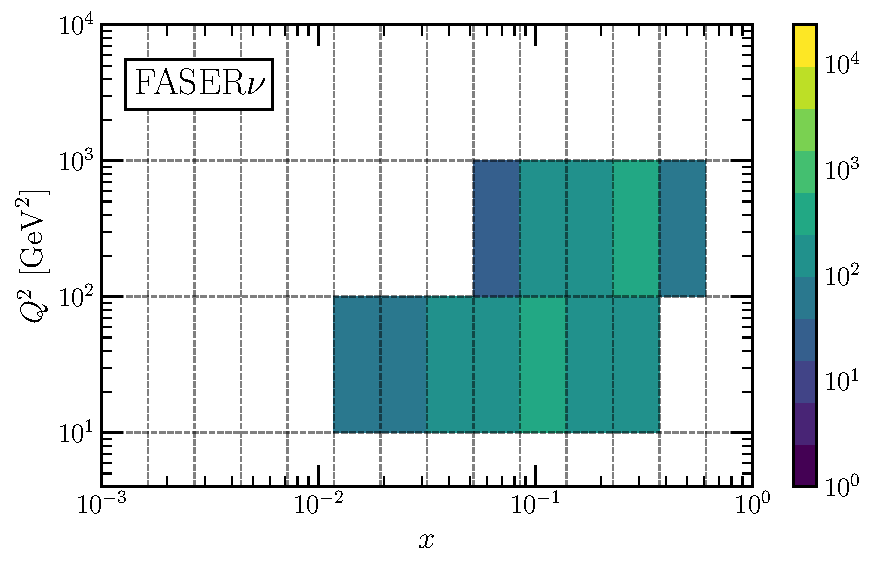
\includegraphics[width=0.495\textwidth]{plots/FPF-FASERv.pdf}
    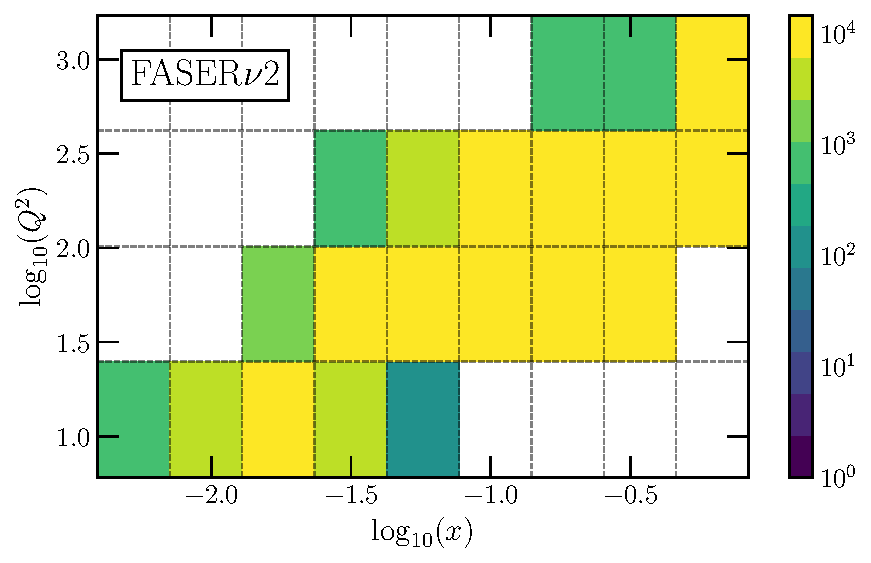
\includegraphics[width=0.495\textwidth]{plots/FPF-FASERv2.pdf}
    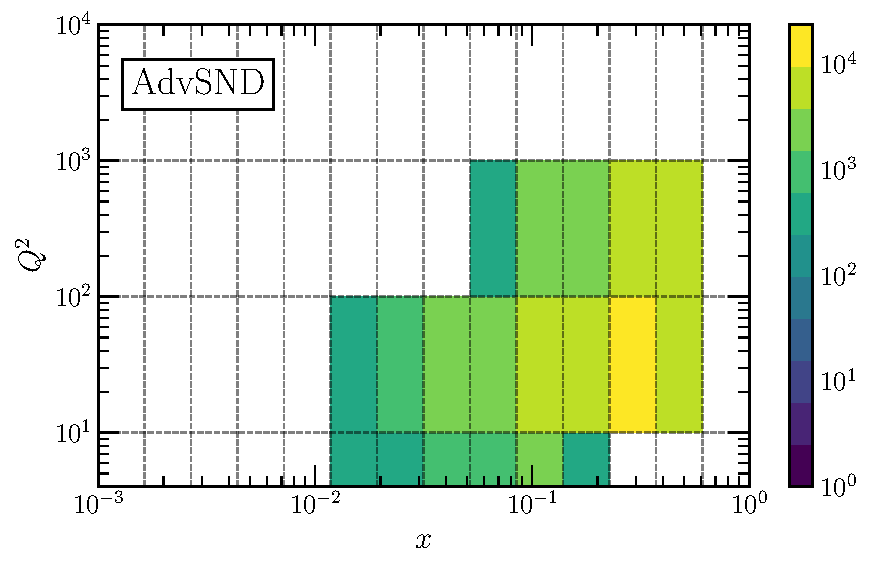
\includegraphics[width=0.495\textwidth]{plots/FPF-AdvSND.pdf}
    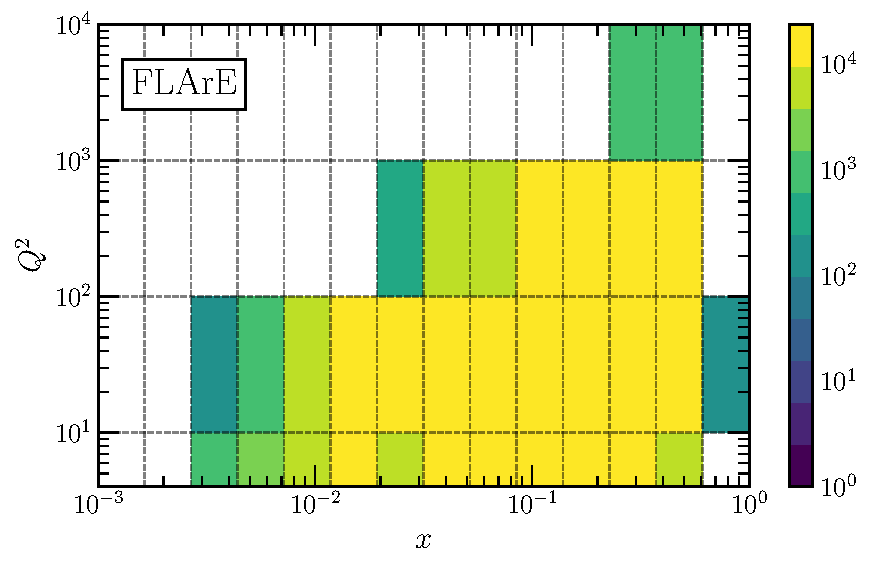
\includegraphics[width=0.495\textwidth]{plots/FPF-FLArE100.pdf}
    \caption{
    	\small The event yields per bin $N_{\rm ev}^{(i)}$,  Eq.~(\ref{eq:event_yields}), for 
    	muon neutrino scattering at the FASER$\nu$, FASER$\nu$2, AdvSND, and FLArE-100  experiments.
        %
   		Selected events are restricted to the DIS region Eq.~(\ref{eq:DISconditions})
   		and only bins with $\ge 100$ events are retained except for FASER$\nu$ in which
   		bins with $\ge 10$ events are kept.
		%
		Adding up the bins in each of the panels results into the numbers listed in
		Table~\ref{tab:integrated_rates}.}
    \label{fig:fasernu2_muon}
\end{figure}
%-----------------------------------------------------------------------

Fig.~\ref{fig:fasernu2_muon} indicates
how the kinematic coverage of the FPF far-forward experiments reaches
$x_{\rm min}\sim 3\times 10^{-3}$ at small-$x$ and $Q^2_{\rm max}\sim 10^4$ GeV$^2$
at large-$Q^2$, representing an extension
of around one order of magnitude in both directions as compared to available
DIS neutrino data on nuclear targets.
%
Fig.~\ref{fig:Kin_nNNPDF30_EIC_FPF} compares
the kinematic coverage of FASER$\nu$, FASER$\nu$2, FLArE, and AdvSND, same as in
Fig.~\ref{fig:fasernu2_muon}, with that of electron-ion collisions
at the upcoming EIC~\cite{Khalek:2021ulf,AbdulKhalek:2021gbh} at the highest
center-of-mass energies planned, as well as to available fixed-target
neutral- and charged-current DIS measurements.
%
The LHC neutrino experiments cover the region $x\gsim 3\times 10^{-3}$, relevant
for precision electroweak measurements at the LHC, such as the $W$-boson
mass, and for new physics measurements sensitive to the large-$x$ quarks
and antiquarks in the proton.
%
FASER$\nu$2 and FLArE-100 mostly overlap with the EIC coverage, providing a complementary handle
on the quark flavour decomposition in protons and heavy nuclei as compared
to that provided by the EIC measurements.

%%%%%%%%%%%%%%%%%%%%%%%%%%%%%%%%%%%%%%%%%%%%%%%%%%%%%
\begin{figure}[t]
    \centering
    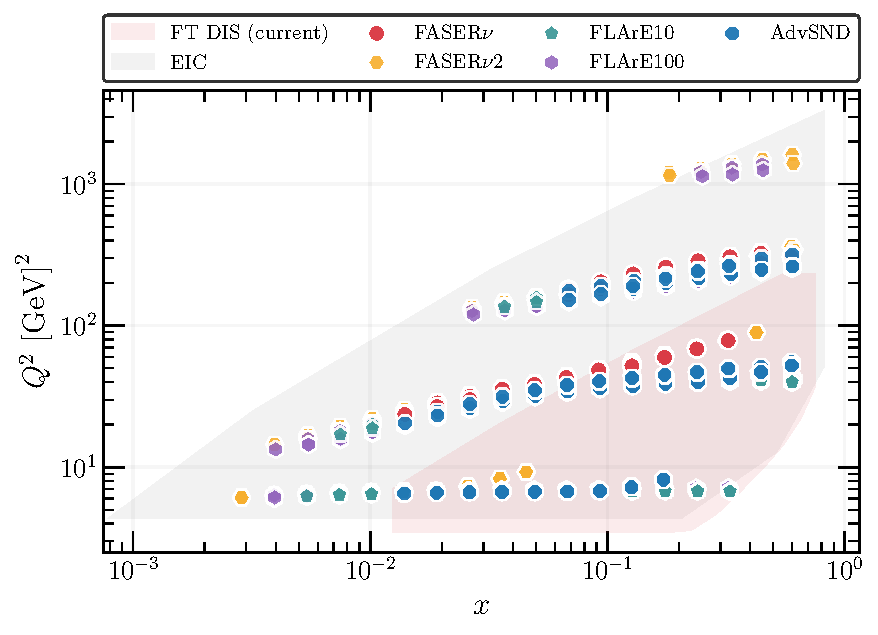
\includegraphics[width = 0.75\textwidth]{plots/KIN_DIS_FPF.pdf}
    \caption{
    	The kinematic coverage in the $(x,Q^2)$ plane of muon-neutrino scattering
	    at the FASER$\nu$, FASER$\nu$2, FLArE-100, and AdvSND experiments, see also Fig.~\ref{fig:fasernu2_muon},
	    compared to that of electron-ion collisions at the EIC for the highest center-of-mass 
	    energies $\sqrt{s}$ planned as well as to the coverage of existing nuclear neutral- and
	    charged-current DIS measurements.
      	%
      	Bins with less than 100 events have been excluded fo all the pseudodata except for FASER$\nu$ where we retain
      	bins with $\ge 10$ events.
  	}
    \label{fig:Kin_nNNPDF30_EIC_FPF}
\end{figure}
%%%%%%%%%%%%%%%%%%%%%%%%%%%%%%%%%%%%%%%%%%%%%%%%%%%%%%%%%%%%%

\subsection{Statistical and systematic uncertainties}
\label{subsec:uncertainties}

The event yields displayed in Fig.~\ref{fig:fasernu2_muon} determine the associated statistical uncertainty 
in each bin,
\be
\label{eq:statistical_uncertainties}
\delta^{\rm (stat)}  N_{\rm ev}^{(i)} = \sqrt{N_{\rm ev}^{(i)}} \, ,
\ee
such that the fractional statistical uncertainty per bin is $\delta^{\rm (stat)}_i=1/\sqrt{N_{\rm ev}^{(i)}}$.
%
Since we discard bins with less than 100 events for HL-LHC experiments (FASER$\nu$2, FLArE100, AdvSND) and
10 events for Run III experiments (FASER$\nu$, SND), the fractional statistical uncertainty
ranges between $\lsim 1\%$ and $\sim 18\%$, depending on the values of
$x$ and $Q^2$ associated to each bin.

%%%%%%%%%%%%%%%%%%%%%%%%%%%%%%%%%%%%%%%%%%%%%%%%%%%%%%%%%%%%%%%%%%%%
\begin{figure}[h]
    \centering
    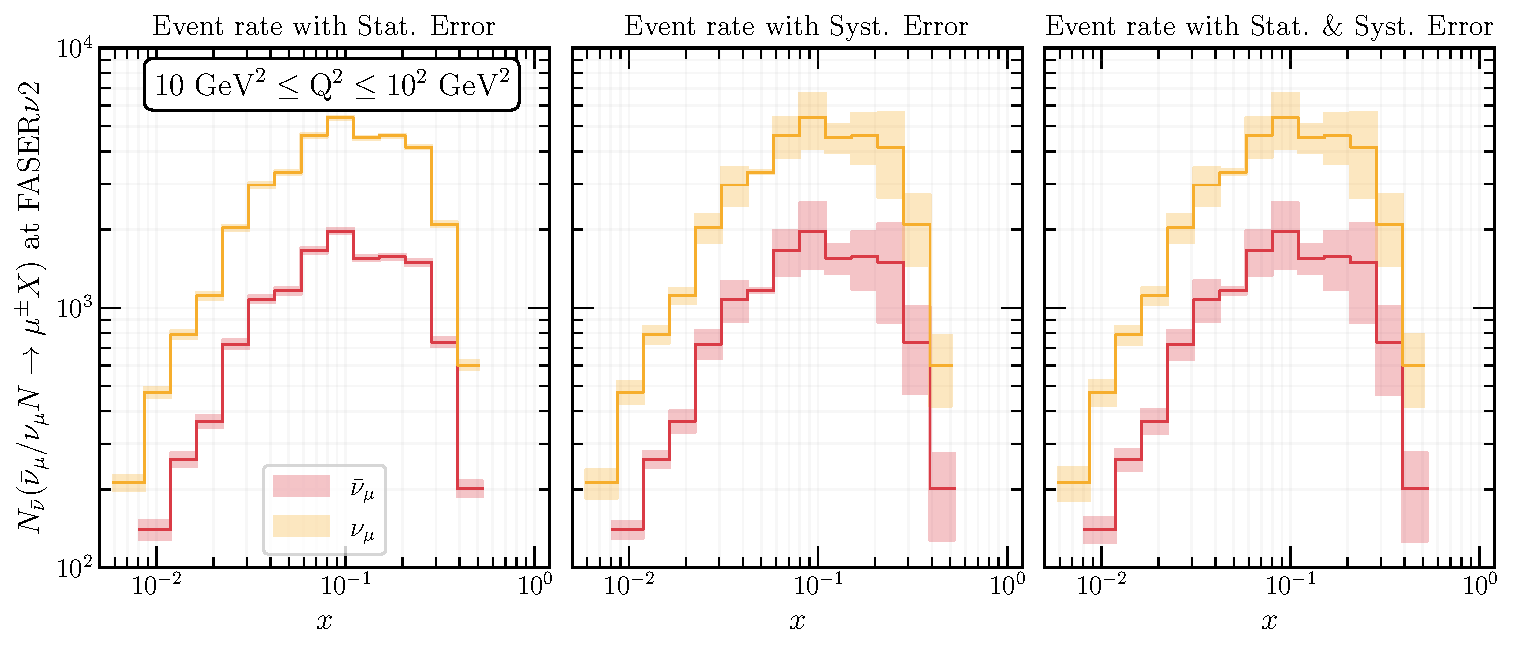
\includegraphics[width = \textwidth]{plots/Event_Rate_FASERv2.pdf}
    \caption{Same as Fig.~\ref{fig:fasernu2_muon} for FASER$\nu$2
      now as a function of $x$ after having integrated the event yields in the range $Q^2 \in [10,100]$ GeV$^2$
      for both the neutrino and antineutrinos.
      %
      In addition to the event yield values, we also show the error bars corresponding to
      statistical errors only (left), systematic errors only (middle), and the
      sum in quadrature of the two (right panel).
      %
      The bars in the horizontal direction indicate the width of the adopted $x$-bins.
      }
    \label{fig:error_plot_FASERv2_14}
\end{figure}
%%%%%%%%%%%%%%%%%%%%%%%%%%%%%%%%%%%%%%%%%%%%%%%%%%%%%%%%%%%%%%%%%%%%

The projected statistical uncertainties for muon-neutrino scattering
in the case of FASER$\nu$2 are displayed in the left panel
of Fig.~\ref{fig:error_plot_FASERv2_14}, which corresponds
to the same event yields as in
Fig.~\ref{fig:fasernu2_muon} for 
now as a function of $x$ after having integrated the event
yields in the range $Q^2 \in [10,100]$ GeV$^2$.
%
The error bar in the vertical direction indicates the statistical uncertainties, while
that in the horizontal direction corresponds to the width of the $x$-bins.
%
Except for the bins with the smallest values of $x$, statistical uncertainties indeed
are at the percent level or smaller for this experiment.

In addition to the statistical uncertainties evaluated from Eq.~(\ref{eq:statistical_uncertainties}),
one needs to also estimate the systematic uncertainties associated to the
finite precision in the reconstruction
of the final state leptonic and hadronic variables listed in Table~\ref{tab:FPF_experiments}.
%
For instance, an event which would be classified into a given bin in $(x,Q^2,E_\nu)$ in the case
of a perfect detector may end up being
mis-classified into a different bin in the presence of systematic
shifts associated to the lepton energy $E_\ell$, lepton scattering angle $\theta_\ell$, and
hadronic energy $E_h$, as indicated by  Eq.~(\ref{eq:dis_kinematic_mapping}).

For each independent source of experimental systematic uncertainty, we hence
quantify its impact at the event yield level.
%
In order to determine these bin-by-bin systematic errors,
we extend the calculation delineated in Eq.~(\ref{sec:pseudo-data_generation}) as follows.
%
Let us consider for illustrative purposes the FASER${\nu}$2 detector.
%
From Table~\ref{tab:FPF_experiments} we know that its
acceptance parameters and reconstruction performance are specified by:
\bea
E_\ell \ge 100~{\rm GeV} \, , \quad \theta_\ell \le \tan^{-1}(0.025)\, , \qquad\\
\delta E_\ell \sim 30\% \, 
 \quad \delta E_h \sim 30\% \, ,
 \quad \delta\theta_\ell \sim 0.06~{\rm mrad} \, . 
\label{eq:fasernu2systematic_errors}
\eea
To translate these uncertainties in $\delta E_\ell$, $\delta E_h $,
and $\delta\theta_\ell$ into systematic errors associated to the event yields, 
\be
\label{eq:event_yields_systematic_error}
\delta_{\rm sys}^{(E_\ell)} N_{\rm ev}^{(i)} \, ,\quad
\delta_{\rm sys}^{(E_h)} N_{\rm ev}^{(i)}
\, ,\quad
\delta_{\rm sys}^{(\theta_\ell)} N_{\rm ev}^{(i)} \, ,\qquad i=1,\ldots,N_{\rm bin} \, ,
\ee
we generate first a Monte Carlo set of events, denoted by $\mathcal{D}_0$,
composed by $N_{\rm mc} \approx 10^7$ samples and determine the assignment of each event
to a point in the $\lp x,Q^2,E_{\nu}\rp$ space.
%
By comparing $\mathcal{D}_0$ with the total number of events as calculated by Eq.~(\ref{MCintegration}), 
we can normalize the distribution to produce the expected yield.

We then produce a second Monte Carlo sample $\mathcal{D}_1$ starting from the events
of $\mathcal{D}_0$ which are then smeared with Gaussian distributions whose variances
are given by Eq.~(\ref{eq:fasernu2systematic_errors}).
%
The bin assignment of the events in the smeared sample $\mathcal{D}_1$ will
in general be different from those of the baseline sample.
%
The procedure is repeated $M$ times, leading to
$\mathcal{D}_k$ (with $k=1,\ldots,M$) smeared
samples each one leading to a different binned event yields
$ N_{\rm ev}^{(i)(k)}$.
%
We take the uncertainty associated
to a given systematic source, say $\delta E_\ell$,
%to be the absolute difference between the mean number of events in this
%bin evaluated for the smeared samples and the
%central prediction for the number of events
to be the mean of the absolute difference between the number of events in this bin for the smeared samples and the central prediction for the number of events
$ N_{\rm ev}^{(i)}$ as calculated from Eq.~(\ref{MCintegration}):
\be
\delta_{\rm sys}^{(E_\ell)} N^{(i)} =\la \Big|  {N}^{(i)}_{E_\ell-{\rm smeared}} -N_{\rm ev}^{(i)}\Big|\ra \, .
\ee

Individual sources of systematic errors are treated as uncorrelated among them and hence
by producing samples where only one source of error is varied at a time
we can determine the systematic errors, Eq.~(\ref{eq:event_yields_systematic_error}), in each bin
for each of the considered experiments.
%
This approach has the benefit that rescaling individual sources of systematic
uncertainties, say to assess the impact of improved detector performance,
becomes straightforward. 

Fig.~\ref{fig:percentage_uncertainties_overview}
displays the projected systematic uncertainties associated
to $E_\ell$, $\theta_\ell$, and $E_h$ 
for the  measurements of the double-differential
muon-neutrino scattering  at FASER$\nu$2.
%
The magnitude of each systematic error is plotted as a function
of the average momentum fraction per bin $\la x\ra$
in two different bins of $Q^2$.
%
We indicate separately the results for neutrino and antineutrino projectiles as well as
those associated to inclusive and to charm production measurements.
%
For completeness, we also display in the bottom-right panel the corresponding
statistical uncertainties in the same bins.

%-----------------------------------------------------------------------
\begin{figure}[t]
  \centering
  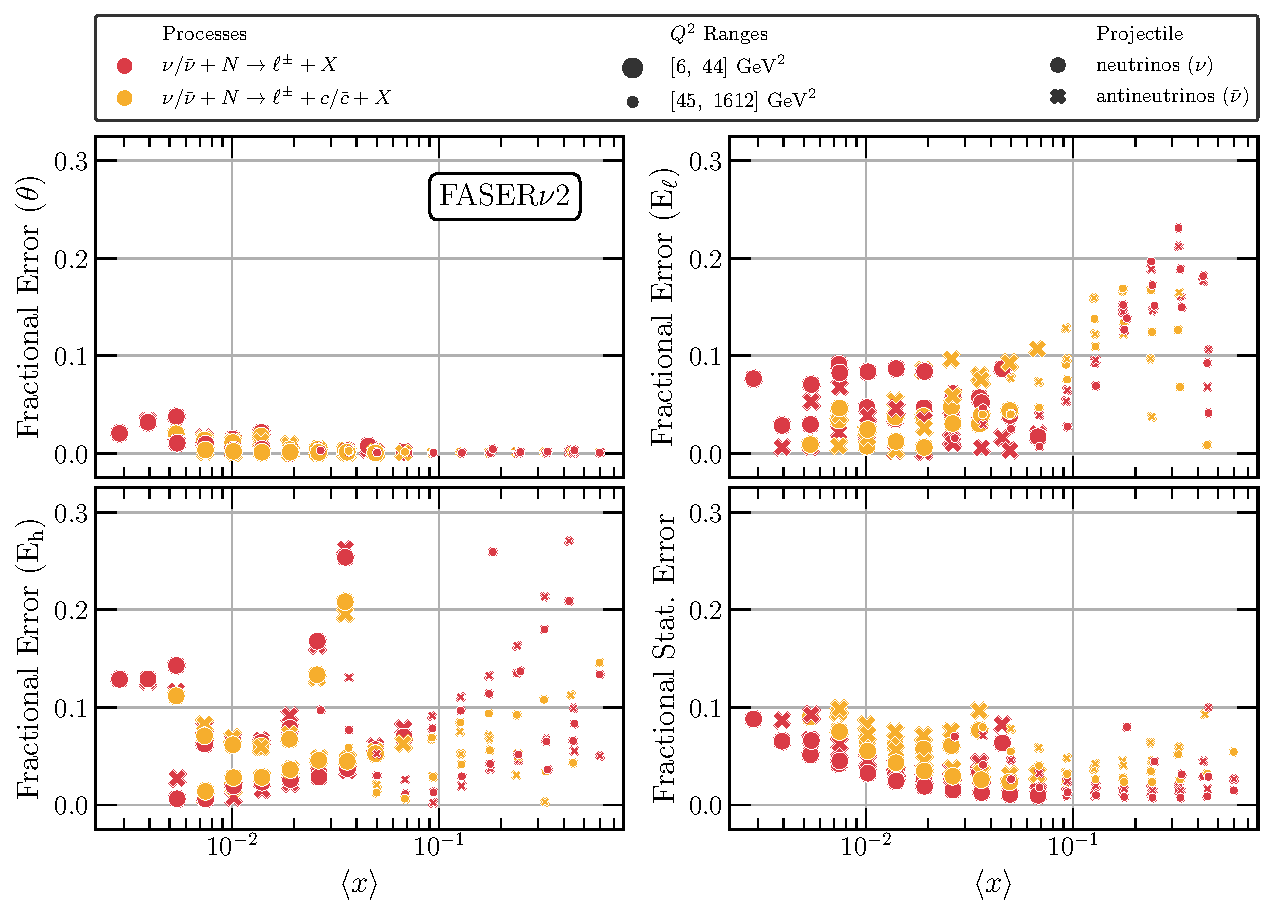
\includegraphics[width=\textwidth]{plots/FASERv2_fractional_error.pdf}
  \caption{\small Estimated systematic uncertainties for the  measurements
    of the double-differential
    muon-neutrino scattering cross-section at FASER$\nu$2.
    %
    We consider the systematic errors
    associated to the charged lepton energy $E_\ell$ and scattering angle $\theta_\ell$
    and to the hadronic energy $E_h$.
    %
    The size of each source of systematic error is plotted as a function
    of the average momentum fraction per bin $\la x\ra$
    in two different bins of $Q^2$.
    %
    We indicate separately the results for neutrino and antineutrino projectiles as well as
    those associated to inclusive and to charm production measurements.
    %
    For completeness, we display in the bottom-right panel the corresponding
    statistical uncertainties in the same bins.
  }
  \label{fig:percentage_uncertainties_overview}
\end{figure}
%-----------------------------------------------------------------------

In general, systematic uncertainties associated to the hadronic final state energy $E_h$ appear to be the largest,
reaching up to $\sim 90\%$ for some experiments.
%
We recall that measurement of $E_h$ in addition to the leptonic variables is required to
fix the incoming neutrino energy $E_\nu$, which is different in each event unlike
the case of neutral-current scattering.
%
The uncertainties associated to the charged-lepton energy $E_\ell$ and scattering angle $\theta_\ell$ range
between a few percent up to 20\% in the  baseline scenario listed in Table~\ref{tab:FPF_experiments}.
%
For the $\delta \theta_\ell$ variations, they are smallest in the large-$x$ region
for $x\gsim 0.1$, where they are at the few-percent level typically.
%
Statistical uncertainties are subdominant in most of the bins and are below the 10\% level,
specially at large-$x$ which is the kinematic region benefitting from the largest event rates.

Fig.~\ref{fig:error_plot_FASERv2_14} also displays
 the integrated event yields for FASER$\nu$2 as a function of $x$ for only
 systematic errors and for the sum in quadrature of statistical and systematic errors
 (central and right panels respectively).
 %
 For most of the bins, for the baseline performance assumptions the total systematic
 uncertainty dominates over the statistical uncertainties, with the possible exception
 of the small-$x$ region where statistical and systematic errors are comparable.

The end result of the procedure is an estimate of statistical and systematic uncertainties
for each bin of the measurement, from which a experimental covariance matrix can be constructed as
\be
\label{eq:covmat_definition}
   {\rm cov}_{ij} = \delta_{ij} \lp \delta^{\rm (stat)}  N_{\rm ev}^{(i)}\rp^2
   + \sum_{k=1}^{n_{\rm sys}}\lp \delta_{\rm sys}^{(k)} N_{\rm ev}^{(i)} \rp \lp \delta_{\rm sys}^{(k)} N_{\rm ev}^{(j)} \rp
   \, ,\qquad i,j=1,\ldots,N_{\rm bin} \, ,
 \ee
  and the same for the associated correlation
 matrix of the measurement
 \be
\label{eq:corrmat_definition}
 \rho_{ij} =  \frac{{\rm cov}_{ij}}{\sqrt{ {\rm cov}_{ii} }\sqrt{ {\rm cov}_{jj} } } \, . 
 \ee
 The relative covariance matrix, $ {\rm cov}_{ij}/( N_{\rm ev}^{(i)}N_{\rm ev}^{(j)})$, is
 independent of the considered observable and would also apply
 for the double-differential cross-sections Eqns.~(\ref{eq:neutrino_DIS_xsec_FL}) and~(\ref{eq:antineutrino_DIS_xsec_FL}) which are related to the event yields by a constant prefactor.
 
 The experimental covariance matrix constructed as per
 Eq.~(\ref{eq:covmat_definition}) assumes that each source of systematic
 uncertainty is 100\% correlated across all the bins of the measurement.
 %
 In the real experiment, the actual covariance matrix will be
 composed by a large number of uncertainty sources, with typical
  HERA and LHC precision measurements characterised by up to hundreds
 of different sources of systematic error.
 %
 In particular, the assumption that a single source of systematic error, say $\delta E_\ell$,
 is fully correlated among all the bins in $(x,Q^2)$ is unlikely to be accurate.
 %
 For this reason, following the HL-LHC projection strategy of~\cite{AbdulKhalek:2018rok}
 here we neglect bin-by-bin correlations
 and add in quadrature statistical and systematic errors,
 \be
\label{eq:covmat_definition_v2}
 {\rm cov}_{ij} = \delta_{ij} \lp \delta^{\rm (stat)}  N_{\rm ev}^{(i)}\rp^2
+ \delta_{ij}\lp f_{\rm corr}\rp^2\sum_{k=1}^{n_{\rm sys}} \lp f_{\rm red}^{(k)}\rp^2\lp \delta_{\rm sys}^{(k)} N_{\rm ev}^{(i)} \rp^2
\, ,\qquad i,j=1,\ldots,N_{\rm bin} \, .
\ee
In Eq.~(\ref{eq:covmat_definition_v2}) we have introduced a parameter $f_{\rm red}^{(k)}\le 1$
that gauges the impact of a possible reduction of the $k$-th systematic error
as compared to the default experiment performance (reproduced with $f_{\rm red}=1$).
%
Furthermore, $f_{\rm corr}$ represents an effective correction factor that accounts for the fact that data with correlated
systematics may be more constraining than the same data where each source of error is simply
added in quadrature as we do here.
%
A value of $f_{\rm corr}=0.5$, obtained from the inspection of available measurements
 for which the full information
 on correlated systematics is available, was estimated in ~\cite{AbdulKhalek:2018rok}
 and we adopt the same choice here.
%
In Sect.~\ref{sec:protonPDFs} we present results for different scenarios
for the systematic uncertainty reduction factor $f_{\rm red}$ with respect to the baseline settings.   
 
 \subsection{Pseudo-data generation}

 In order to generate pseudo-data for double-differential
 LHC neutrino scattering cross-sections, we follow the procedure
 used for the HL-LHC projections of~\cite{AbdulKhalek:2018rok} which was
 also adopted in~\cite{Ethier:2021ydt} and~\cite{Greljo:2021kvv} for SMEFT impact projections
 of vector-boson scattering and high-mass Drell-Yan data at the HL-LHC, respectively.
 %
 The starting point are predictions for inclusive and charm-tagged
 differential neutrino scattering cross-section, denoted generically by
 \be
 \label{eq:theory_dis_projections}
 \mathcal{O}_i^{{\rm (th)}} \equiv \frac{d^2\sigma^{\nu N}(x_i,Q^2_i,y_i)}{dxdy} \, ,\quad
 i=1,\ldots,N_{\rm bin} \, ,
 \ee
 with $(x_i,Q^2_i,y_i)$ labeling the corresponding bin centers.
 %
 The observables $\mathcal{O}_i $ in Eq.~(\ref{eq:theory_dis_projections})
are evaluated with the
{\sc\small YADISM}~\cite{yadism,Candido:2023utz} program
interfaced to {\sc\small PineAPPL}~\cite{Carrazza:2020gss, christopher_schwan_2023_7995675}
to return a fast interpolation grid admitting a generic PDF input,
and with DGLAP evolution effects provided by {\sc\small EKO}~\cite{Candido:2022tld}.
%
PDF evolution and DIS structure functions account for NLO QCD corrections
and target mass effects.
%
No higher-twists corrections are included.
%
Charm structure functions are evaluated in the FONLL general-mass variable-flavour-number
scheme~\cite{Forte:2010ta,Ball:2011mu,Faura:2020oom} at $\mathcal{O}\lp \alpha_s\rp$
accuracy.
%
For the proton PDF fits we assume a free isoscalar target $N$, while
for the nuclear PDF one we allow for deviations from isoscalarity relevant
for a tungsten nucleus.

The PDF set and other theory settings, such as the perturbative
order and heavy quark scheme, adopted for the evaluation of
Eq.~(\ref{eq:theory_dis_projections}) should be the same as those
used in the fitting framework assessing their impact.
%
For instance, when using the {\sc\small xFitter} profiling of PDF4LHC21, one needs
 to generate LHC neutrino pseudo-data also using PDF4LHC21 as input.
 %
This ensures that the generated pseudo-data is consistent with the prior PDF
 set used as baseline and avoids introducing artificial inconsistencies 
 compromising the validity of the projection studies.
 
 The central values for the pseudo-data, denoted
 by $\mathcal{O}_i^{{\rm (exp)}} $, are obtained
 by fluctuating the reference theory prediction Eq.~(\ref{eq:theory_dis_projections})
 by the corresponding fractional statistical and systematic
 uncertainties,
 \begin{equation}
  \label{eq:pseudo_data_v2}
  \mathcal{O}_i^{{\rm (exp)}}
  = \mathcal{O}_i^{{\rm (th)}}
    \left( 1+ r_i \delta_i^{\rm tot}
    \right) \,
    , \qquad i=1,\ldots,N_{\rm bin} \, ,
 \end{equation}
 where the total experimental uncertainty is the sum in quadrature of
 statistical and systematic errors, accounting for a possible reduction
 factor in the latter,
  \be
 \delta_{i}^{\rm tot}
 = \left( \left( \delta_i^{\rm stat}\right)^2 + \sum_{k=1}^{n_{\rm sys}}
 \left( f_{\rm corr} \times f_{\rm red}^{(k)} \times \delta_{i,k}^{\rm sys} \right)^2\right)^{1/2} \, ,
 \qquad i=1,\ldots,N_{\rm bin} \, ,
 \ee
 and with $r_{i}$ being univariate Gaussian random numbers. 
 %
 As mentioned above, $f_{\rm red}^{(k)}$ is a reduction factor modelling
 improvements in the experimental performance as compared to the baseline
 settings summarised in Sect.~\ref{tab:FPF_experiments}.
 %
 Here we consider two scenarios for the systematic errors: ``conservative'',  with $f_{\rm red}=1$, where
 no improvement as compared to current projected performance takes place, and ``optimistic'', with  $f_{\rm red}=0.5$, a factor
 two improvement for all sources of systematics.
 %
 The pseudo-data generated by means of Eq.~(\ref{eq:pseudo_data_v2}),
 together with the corresponding covariance matrix computed according to Eq.~\eqref{eq:covmat_definition_v2},
 define then the inputs of the subsequent proton and nuclear PDF determination.

 \subsection{PDF impact assessment}
 \label{subsec:pdf_impact_assessment}

We consider two complementary approaches to assess the
impact of the projected LHC neutrino data on the proton and nuclear PDFs.
%
First, the Hessian profiling\cite{Paukkunen:2014zia, Schmidt:2018hvu, AbdulKhalek:2018rok, HERAFitterdevelopersTeam:2015cre} of prior proton and
nuclear PDF sets, taken to be PDF4LHC21~\cite{PDF4LHCWorkingGroup:2022cjn} and
EPPS21~\cite{Eskola:2021nhw} respectively.
%
Second, the direct inclusion 
in the NNPDF global analysis framework~\cite{NNPDF:2021uiq,NNPDF:2021njg}.
%
The profiling method applied to Hessian PDF fits is based
on minimizing a goodness-of-fit error function defined as
\begin{equation}
\chi^2 = 
\sum_{i=1}^{N_{\textrm{bin}}} 
\frac{\left(  \mathcal{O}_i^{\rm (exp)}
            + \Gamma_i^{\alpha,\textrm{exp}}
              b_\alpha^{\textrm{(exp)}}
            - \mathcal{O}_i^{\rm (th)}
            - \Gamma_i^{\beta,\textrm{th}}
              b_\beta^{(\textrm{th})}
     \right)^2
     }{ \left(\delta^{{\rm (stat)}}\mathcal{O}_i^{\rm (th)}\rp^2 }
+ \sum_\alpha \lp b_\alpha^{(\textrm{exp})}\rp^2
+ T^2 \sum_\beta  \lp b_\beta^{\textrm{(th)}}\rp ^2 \, ,
\label{eq:profilingchi2}
\end{equation}
with the pseudodata 
$\mathcal{O}_i^{\rm (exp)}$ defined in  Eq.~(\ref{eq:pseudo_data_v2}).
%
The correlated uncertainties for the pseudodata and for the theoretical prediction 
are contained in the nuisance parameter vectors $b^{(\textrm{exp})}$ and $b^{(\textrm{th})}$, respectively, with $T$ the tolerance factor, and the total uncorrelated uncertainty is $\delta^{{\rm (stat)}}\mathcal{O}_i^{\rm (th)}$.

The effect of the nuisance parameters
on the observables $\mathcal{O}_i^{\rm (exp)}$ and $\mathcal{O}_i^{\rm (th)}$
is described by the matrices $\Gamma_i^{\textrm{exp}}$ and $\Gamma_i^{\textrm{th}}$.
%
The indices $\alpha$ and $\beta$ then run over the uncertainty nuisance parameters for the pseudodata and the theoretical prediction, respectively.
%
The nuisance parameter values $b_\beta^{\textrm{(th,min)}}$ that minimize Eq.~\eqref{eq:profilingchi2} give the central PDFs $f'_0$ optimized to the profiled dataset in the form
\begin{equation}
f_0' = f_0
      + \sum_\beta b_\beta^{\textrm{(th,min)}} 
        \left(  \frac{f_\beta^+   -  f_\beta^- }{2}
              -    b_\beta^{\textrm{(th,min)}}
                \frac{f_\beta^+ + f_\beta^- - 2f_0}{2}
        \right),
\end{equation}
where $f_0$ is the original central PDF and the up and down variation eigenvectors are given by $f^+, f^-$.
%
The reduction in the uncertainties of the profiled PDFs indicate the impact
of the projected data with respect to the assumed prior PDF set.

The profiling studies carried out in this work are performed using version 2.2.1
of the 
{\sc\small xFitter} open-source QCD analysis framework~\cite{Alekhin:2014irh, Bertone:2017tig, xFitter:2022zjb, xFitter:web}.
%
To this end, a new interface between  {\sc\small PineAPPL} and {\sc\small xFitter} has been developed and is available in {\sc\small xFitter}.
%
All the experimental and theoretical data files used in the analysis, including
the  {\sc\small PineAPPL}  grids, are available
from the {\sc\small xFitter} repository.
%
For the proton PDF profiling, a tolerance of $T^2 = 10$ is adopted,
which  corresponds approximately to the average tolerance
used in the CT18~\cite{Hou:2019efy} and MSHT20~\cite{Bailey:2020ooq} determinations,
the two Hessian sets entering the PDF4LHC21 combination~\cite{PDF4LHCWorkingGroup:2022cjn}, for
one-sigma PDF uncertainties.
%
For the Hessian profiling of EPPS21, a value of $T^2 = 20$ is used consistently with~\cite{Eskola:2021nhw}
for the definition of 68\%  confidence level intervals.

Concerning the inclusion of the LHC far-forward neutrino pseudo-data
in the NNPDF proton analysis framework, we follow the procedure
outlined in~\cite{NNPDF:2021uiq}.
%
Fast interpolation tables (FK-tables)~\cite{Ball:2010de} combining {\sc\small EKO}
DGLAP evolution with {\sc\small YADISM} DIS coefficient functions
are computed using {\sc\small PineAPPL}, see also~\cite{Barontini:2023vmr}.
%
Predictions for the observables Eq.~(\ref{eq:theory_dis_projections}) are evaluated
with NNPDF4.0 NNLO for various choices of input datasets, and included
directly in the same alongside all other datasets in the global fit.
%
We verify that in all cases $\chi^2/n_{\rm dat}\sim 1$ after the fit,
as expected given the built-in consistency between the prior PDF fit
and the generated pseudo-data.
%
We assess the impact of the forward LHC neutrino data in the NNPDF fits both when added
on top of the baseline dataset and when added to a dataset which excludes previous neutrino DIS
cross-section measurements.




